\section{Verification}
\label{section: Chapter3/verification}

%%%%%%%%%%%%%%%%%%%%%%%%%%%%%%%%%%%%%%%%%%%%%%%%%%%%%%%%%%%%%%%%%%%%%%%%%%%%%%%%%%%%%%%%%%%
%%%%%%%%%%%%%%%%%%%%%%%%%%%%%%%%%%%%%%%%%%%%%%%%%%%%%%%%%%%%%%%%%%%%%%%%%%%%%%%%%%%%%%%%%%%
%%%%%%%%%%%%%%%%%%%%%%%%%%%%%%%%%%%%%%%%%%%%%%%%%%%%%%%%%%%%%%%%%%%%%%%%%%%%%%%%%%%%%%%%%%%
%%%%%%%%%%%%%%%%%%%%%%%%%%%%%%%%%%%%%%%%%%%%%%%%%%%%%%%%%%%%%%%%%%%%%%%%%%%%%%%%%%%%%%%%%%%
%%%%%%%%%%%%%%%%%%%%%%%%%%%%%%%%%%%%%%%%%%%%%%%%%%%%%%%%%%%%%%%%%%%%%%%%%%%%%%%%%%%%%%%%%%%
%%%%%%%%%%%%%%%%%%%%%%%%%%%%%%%%%%%%%%%%%%%%%%%%%%%%%%%%%%%%%%%%%%%%%%%%%%%%%%%%%%%%%%%%%%%
%%%%%%%%%%%%%%%%%%%%%%%%%%%%%%%%%%%%%%%%%%%%%%%%%%%%%%%%%%%%%%%%%%%%%%%%%%%%%%%%%%%%%%%%%%%
%%%%%%%%%%%%%%%%%%%%%%%%%%%%%%%%%%%%%%%%%%%%%%%%%%%%%%%%%%%%%%%%%%%%%%%%%%%%%%%%%%%%%%%%%%%
%%%%%%%%%%%%%%%%%%%%%%%%%%%%%%%%%%%%%%%%%%%%%%%%%%%%%%%%%%%%%%%%%%%%%%%%%%%%%%%%%%%%%%%%%%%
%%%%%%%%%%%%%%%%%%%%%%%%%%%%%%%%%%%%%%%%%%%%%%%%%%%%%%%%%%%%%%%%%%%%%%%%%%%%%%%%%%%%%%%%%%%
\subsection{Uniaxial traction of a bar}
\label{section: Chapter3/verification/bar}

We first verify the uniaxial response of the quasi-brittle fracture model with pressurization. Consider a bar of length $L = \SI{400}{\milli\meter}$ and width $W = \SI{2}{\milli\meter}$ that is subject to uniaxial tension. Plane strain conditions are assumed to hold. A similar example without crack pressurization can be found in \cite{JYWu2017}. Boundary conditions are shown in \Cref{fig:bar}. Both ends of the bar are subject to monotonically increasing horizontal displacements. Only a quarter of the domain is simulated utilizing the two symmetry conditions. The domain is uniformly discretized using \texttt{QUAD4} elements, with 200 elements along the length and 1 element along the width. Included are the Young's modulus $E = \SI{3e4}{\mega\pascal}$, Poisson's ratio $\nu = 0.2$, critical fracture strength $\psi_c = \SI{1.5e-4}{\milli\joule\per\cubic\milli\meter}$, fracture toughness $\Gc = \SI{0.12}{\milli\joule\per\square\milli\meter}$, and the Griffith’s characteristic length $l_\text{ch} = \dfrac{\Gc}{2\psi_c} = \SI{400}{\milli\meter}$.

\begin{figure}[!ht]
  \centering
  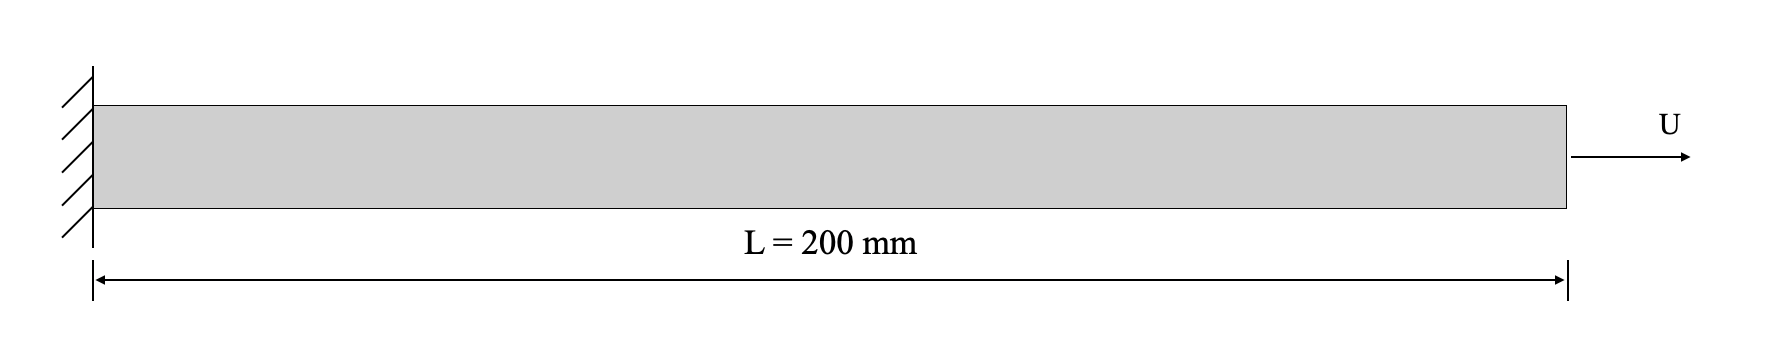
\includegraphics[width=0.9\textwidth,trim={0 8cm 0 8cm},clip]{Chapter3/figures/bar}
  \caption{A bar under uniaxial tension.}
  \label{fig:bar}
\end{figure}

An arbitrarily small imperfection, $d_0 = \mathcal{O}(\epsilon)$, is introduced on the left side of the computational domain to induce localization.
To study the effect of the pressure, different pressure values
\begin{align*}
  \bar{p} \in \left\{ \SI{0.2}{\mega\pascal}, \SI{0.4}{\mega\pascal}, \SI{0.6}{\mega\pascal}, \SI{0.8}{\mega\pascal}, \SI{1}{\mega\pascal} \right\}
\end{align*}
are considered, with a fixed phase-field regularization length of $l = \SI{20}{\milli\meter}$. In the context of fuel fracture, the pressure on the crack surfaces can result from a pressurized gas environment. The reaction force on the left boundary in \Cref{fig:bar_pressure} shows that softening occurs simultaneously for different pressure values. With a larger pressure value, the damage grows more quickly.
As is seen in \Cref{fig:bar_pressure_right}, the reaction force on the right boundary is balanced with the prescribed pressure once the crack has fully developed. \Cref{fig:bar_pressure_only} plots the approximated effective pressure $\widetilde{p}$ \eqref{eq:pressure_approx}, which shows good agreement with prescribed values $\bar{p}$.

\begin{figure}[htb!]
  \centering
  \begin{subfigure}[t]{0.49\linewidth}
    \centering
    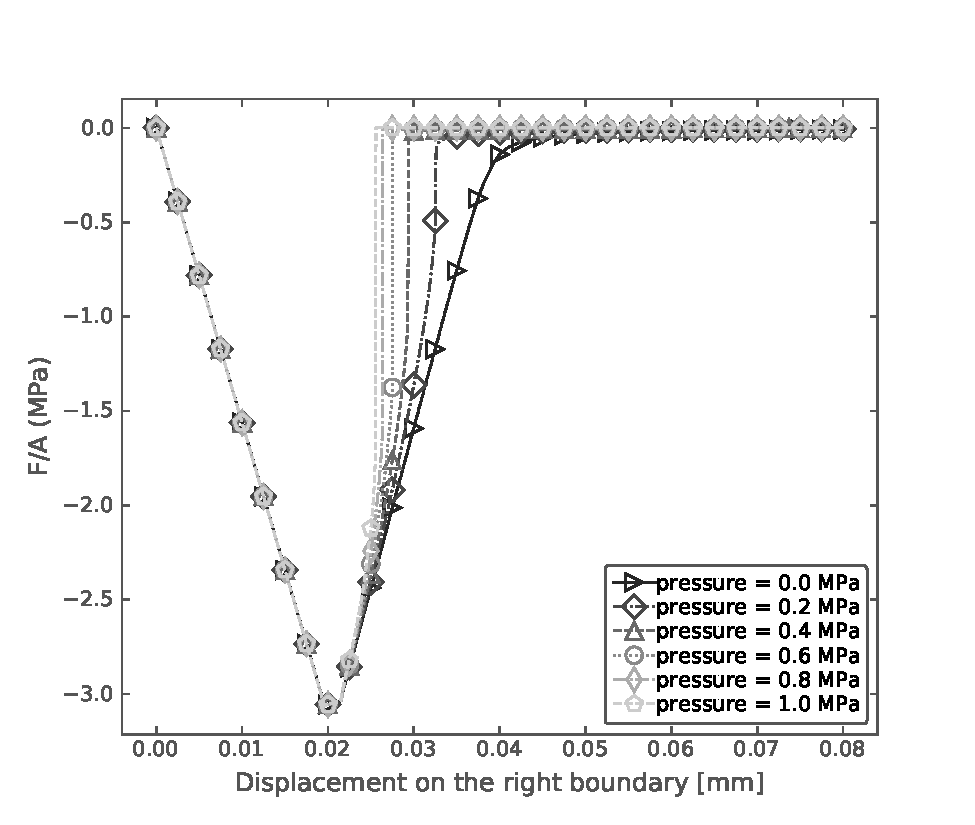
\includegraphics[width=\linewidth]{Chapter3/figures/bar_pressure_left}
    \caption{}
    \label{fig:bar_pressure}
  \end{subfigure}
  \begin{subfigure}[t]{0.49\linewidth}
    \centering
    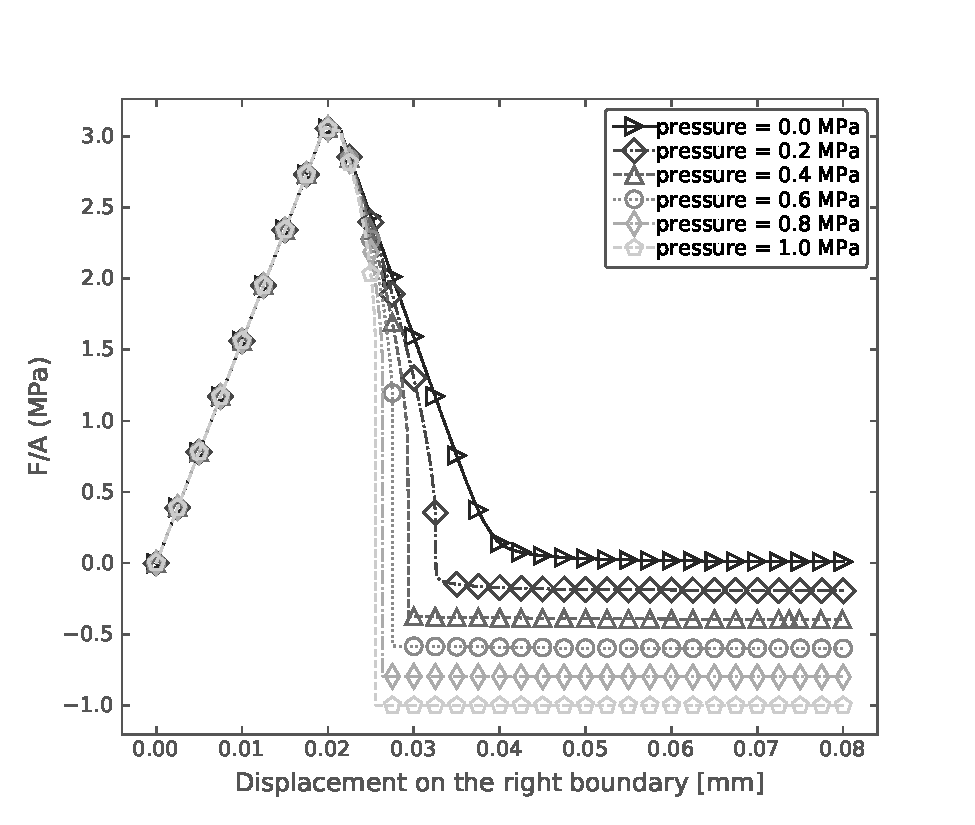
\includegraphics[width=\linewidth]{Chapter3/figures/bar_pressure_right}
    \caption{}
    \label{fig:bar_pressure_right}
  \end{subfigure}
  \begin{subfigure}[t]{0.49\linewidth}
    \centering
    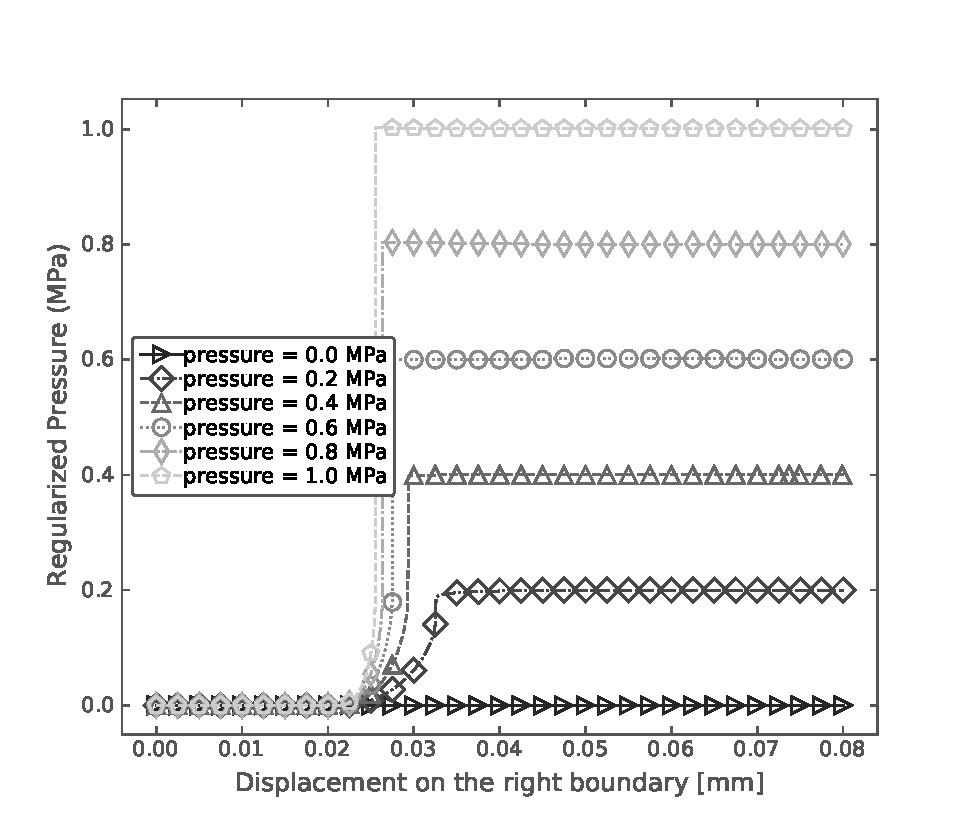
\includegraphics[width=\linewidth]{Chapter3/figures/bar_pressure_only}
    \caption{}
    \label{fig:bar_pressure_only}
  \end{subfigure}
  \caption{\label{fig:bar_pressure_all} A bar under uniaxial tension with different pressure values $\bar{p}$: (a) Reaction force on the left boundary. (b) Reaction force on the right boundary. (c) Regularized pressure value.}
\end{figure}

\citet{JYWu2017} demonstrated that the numerical results are independent of the phase-field regularization length for a quasi-brittle fracture model without pressure \cite{JYWu2017}. Here, we consider a series of values of phase-field regularization length
\begin{align*}
  l \in \left\{ \SI{5}{\milli\meter}, \SI{10}{\milli\meter}, \SI{20}{\milli\meter}, \SI{50}{\milli\meter} \right\}
\end{align*}
with a fixed pressure of $\bar{p}=\SI{0.4}{\mega\pascal}$. \Cref{fig:bar_length} reveals the softening behaviors to be essentially the same, regardless of the chosen regularization length $l$. This feature allows for choosing $\Gc$ and $\psi_c$ values independently from the regularization length.

\begin{figure}[!ht]
  \centering
  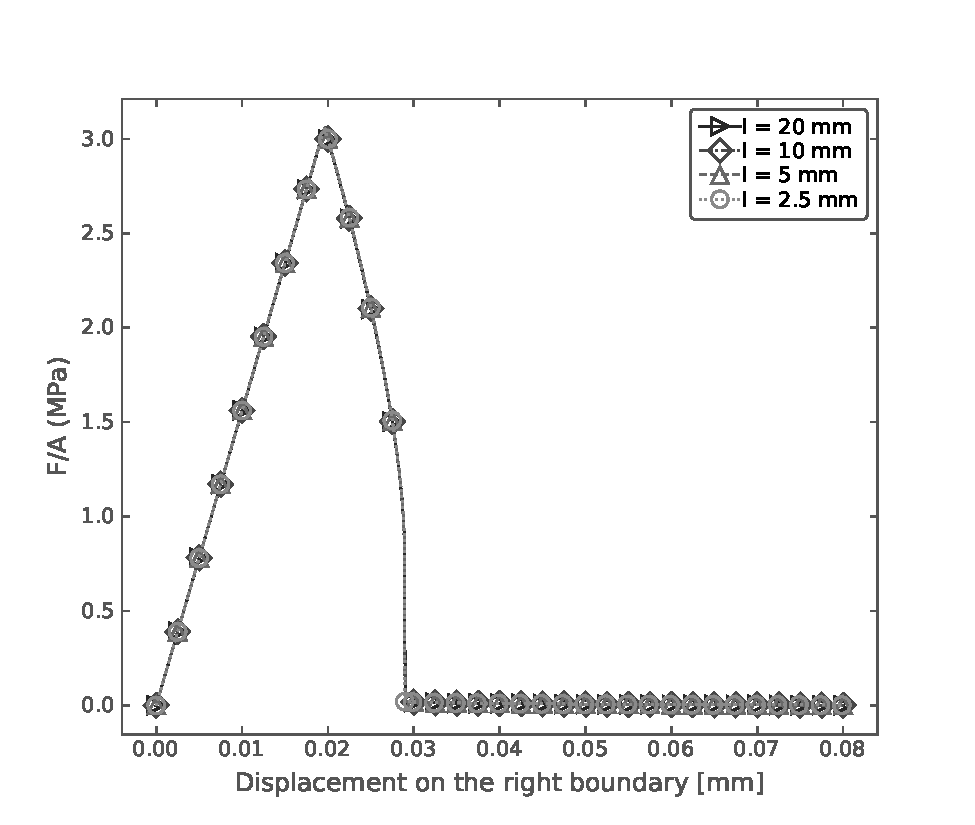
\includegraphics[width=0.6\textwidth]{Chapter3/figures/bar_length}
  \caption{A bar under uniaxial tension with different internal lengths $l$.}
  \label{fig:bar_length}
\end{figure}

%%%%%%%%%%%%%%%%%%%%%%%%%%%%%%%%%%%%%%%%%%%%%%%%%%%%%%%%%%%%%%%%%%%%%%%%%%%%%%%%%%%%%%%%%%%
%%%%%%%%%%%%%%%%%%%%%%%%%%%%%%%%%%%%%%%%%%%%%%%%%%%%%%%%%%%%%%%%%%%%%%%%%%%%%%%%%%%%%%%%%%%
%%%%%%%%%%%%%%%%%%%%%%%%%%%%%%%%%%%%%%%%%%%%%%%%%%%%%%%%%%%%%%%%%%%%%%%%%%%%%%%%%%%%%%%%%%%
%%%%%%%%%%%%%%%%%%%%%%%%%%%%%%%%%%%%%%%%%%%%%%%%%%%%%%%%%%%%%%%%%%%%%%%%%%%%%%%%%%%%%%%%%%%
%%%%%%%%%%%%%%%%%%%%%%%%%%%%%%%%%%%%%%%%%%%%%%%%%%%%%%%%%%%%%%%%%%%%%%%%%%%%%%%%%%%%%%%%%%%
%%%%%%%%%%%%%%%%%%%%%%%%%%%%%%%%%%%%%%%%%%%%%%%%%%%%%%%%%%%%%%%%%%%%%%%%%%%%%%%%%%%%%%%%%%%
%%%%%%%%%%%%%%%%%%%%%%%%%%%%%%%%%%%%%%%%%%%%%%%%%%%%%%%%%%%%%%%%%%%%%%%%%%%%%%%%%%%%%%%%%%%
%%%%%%%%%%%%%%%%%%%%%%%%%%%%%%%%%%%%%%%%%%%%%%%%%%%%%%%%%%%%%%%%%%%%%%%%%%%%%%%%%%%%%%%%%%%
%%%%%%%%%%%%%%%%%%%%%%%%%%%%%%%%%%%%%%%%%%%%%%%%%%%%%%%%%%%%%%%%%%%%%%%%%%%%%%%%%%%%%%%%%%%
%%%%%%%%%%%%%%%%%%%%%%%%%%%%%%%%%%%%%%%%%%%%%%%%%%%%%%%%%%%%%%%%%%%%%%%%%%%%%%%%%%%%%%%%%%%
\subsection{Pressurized crack propagation}
\label{section: Chapter3/verification/propagation}

Next, we verify fracture propagation conditions predicted by the quasi-brittle fracture model using a benchmark problem proposed by \citet{WILSON2016264}. This problem serves to verify whether cracks should propagate once a critical pressure loading is applied. In \Cref{fig:sneddon_c}, an initial crack is prescribed in the center with a length of $2a$. As shown in \Cref{fig:sneddon_c0}, the phase-field is initialized to be 1.0 only for those nodes on the bottom boundary belonging to the crack set, the phase-field variable is regularized to satisfy the governing equations, as shown in \Cref{fig:sneddon_c1}. Note that this differs from the approach suggested in \cite{WILSON2016264,YOSHIOKA2020113210} which involves imposing initial values for a set of elements.
Utilizing the symmetry, only half of the domain with size $L \times L/2$ is used (\Cref{fig:sneddon_mesh}). The ratio $L/a$ is taken to be 20. All outer surfaces are fixed. A prescribed pressure is increased until the crack starts to propagate. The propagation of the crack right after the critical pressure is attained is unstable. According to the linear elastic fracture mechanics (LEFM) solution, the normalized critical pressure is given as:
\begin{equation}
  \dfrac{p_c}{\sigma_0} = \sqrt{\dfrac{l}{\pi a}}, \quad \sigma_0=\sqrt{\dfrac{E}{(1-\nu^2)} \dfrac{\Gc^\text{eff}}{l}},
\end{equation}
where $\Gc^\text{eff}$ is the effective fracture toughness in the phase-field fracture model and is given as \cite{Bourding2008,YOSHIOKA2020113210}:
\begin{equation}
  \Gc^\text{eff} = \Gc\left(\dfrac{h}{4c_0l}+1\right).
\end{equation}
Note that the LEFM solution is based on a brittle fracture model. A comparison between the numerical results and the LEFM solution for the critical pressure values is shown in \Cref{fig:critical_presssure}. The phase-field solution converges as $\psi_c$ increases, and shows good agreement with the LEFM solution.

\begin{figure}[htbp!]
  \centering
  \begin{subfigure}[t]{0.46\linewidth}
    \centering
    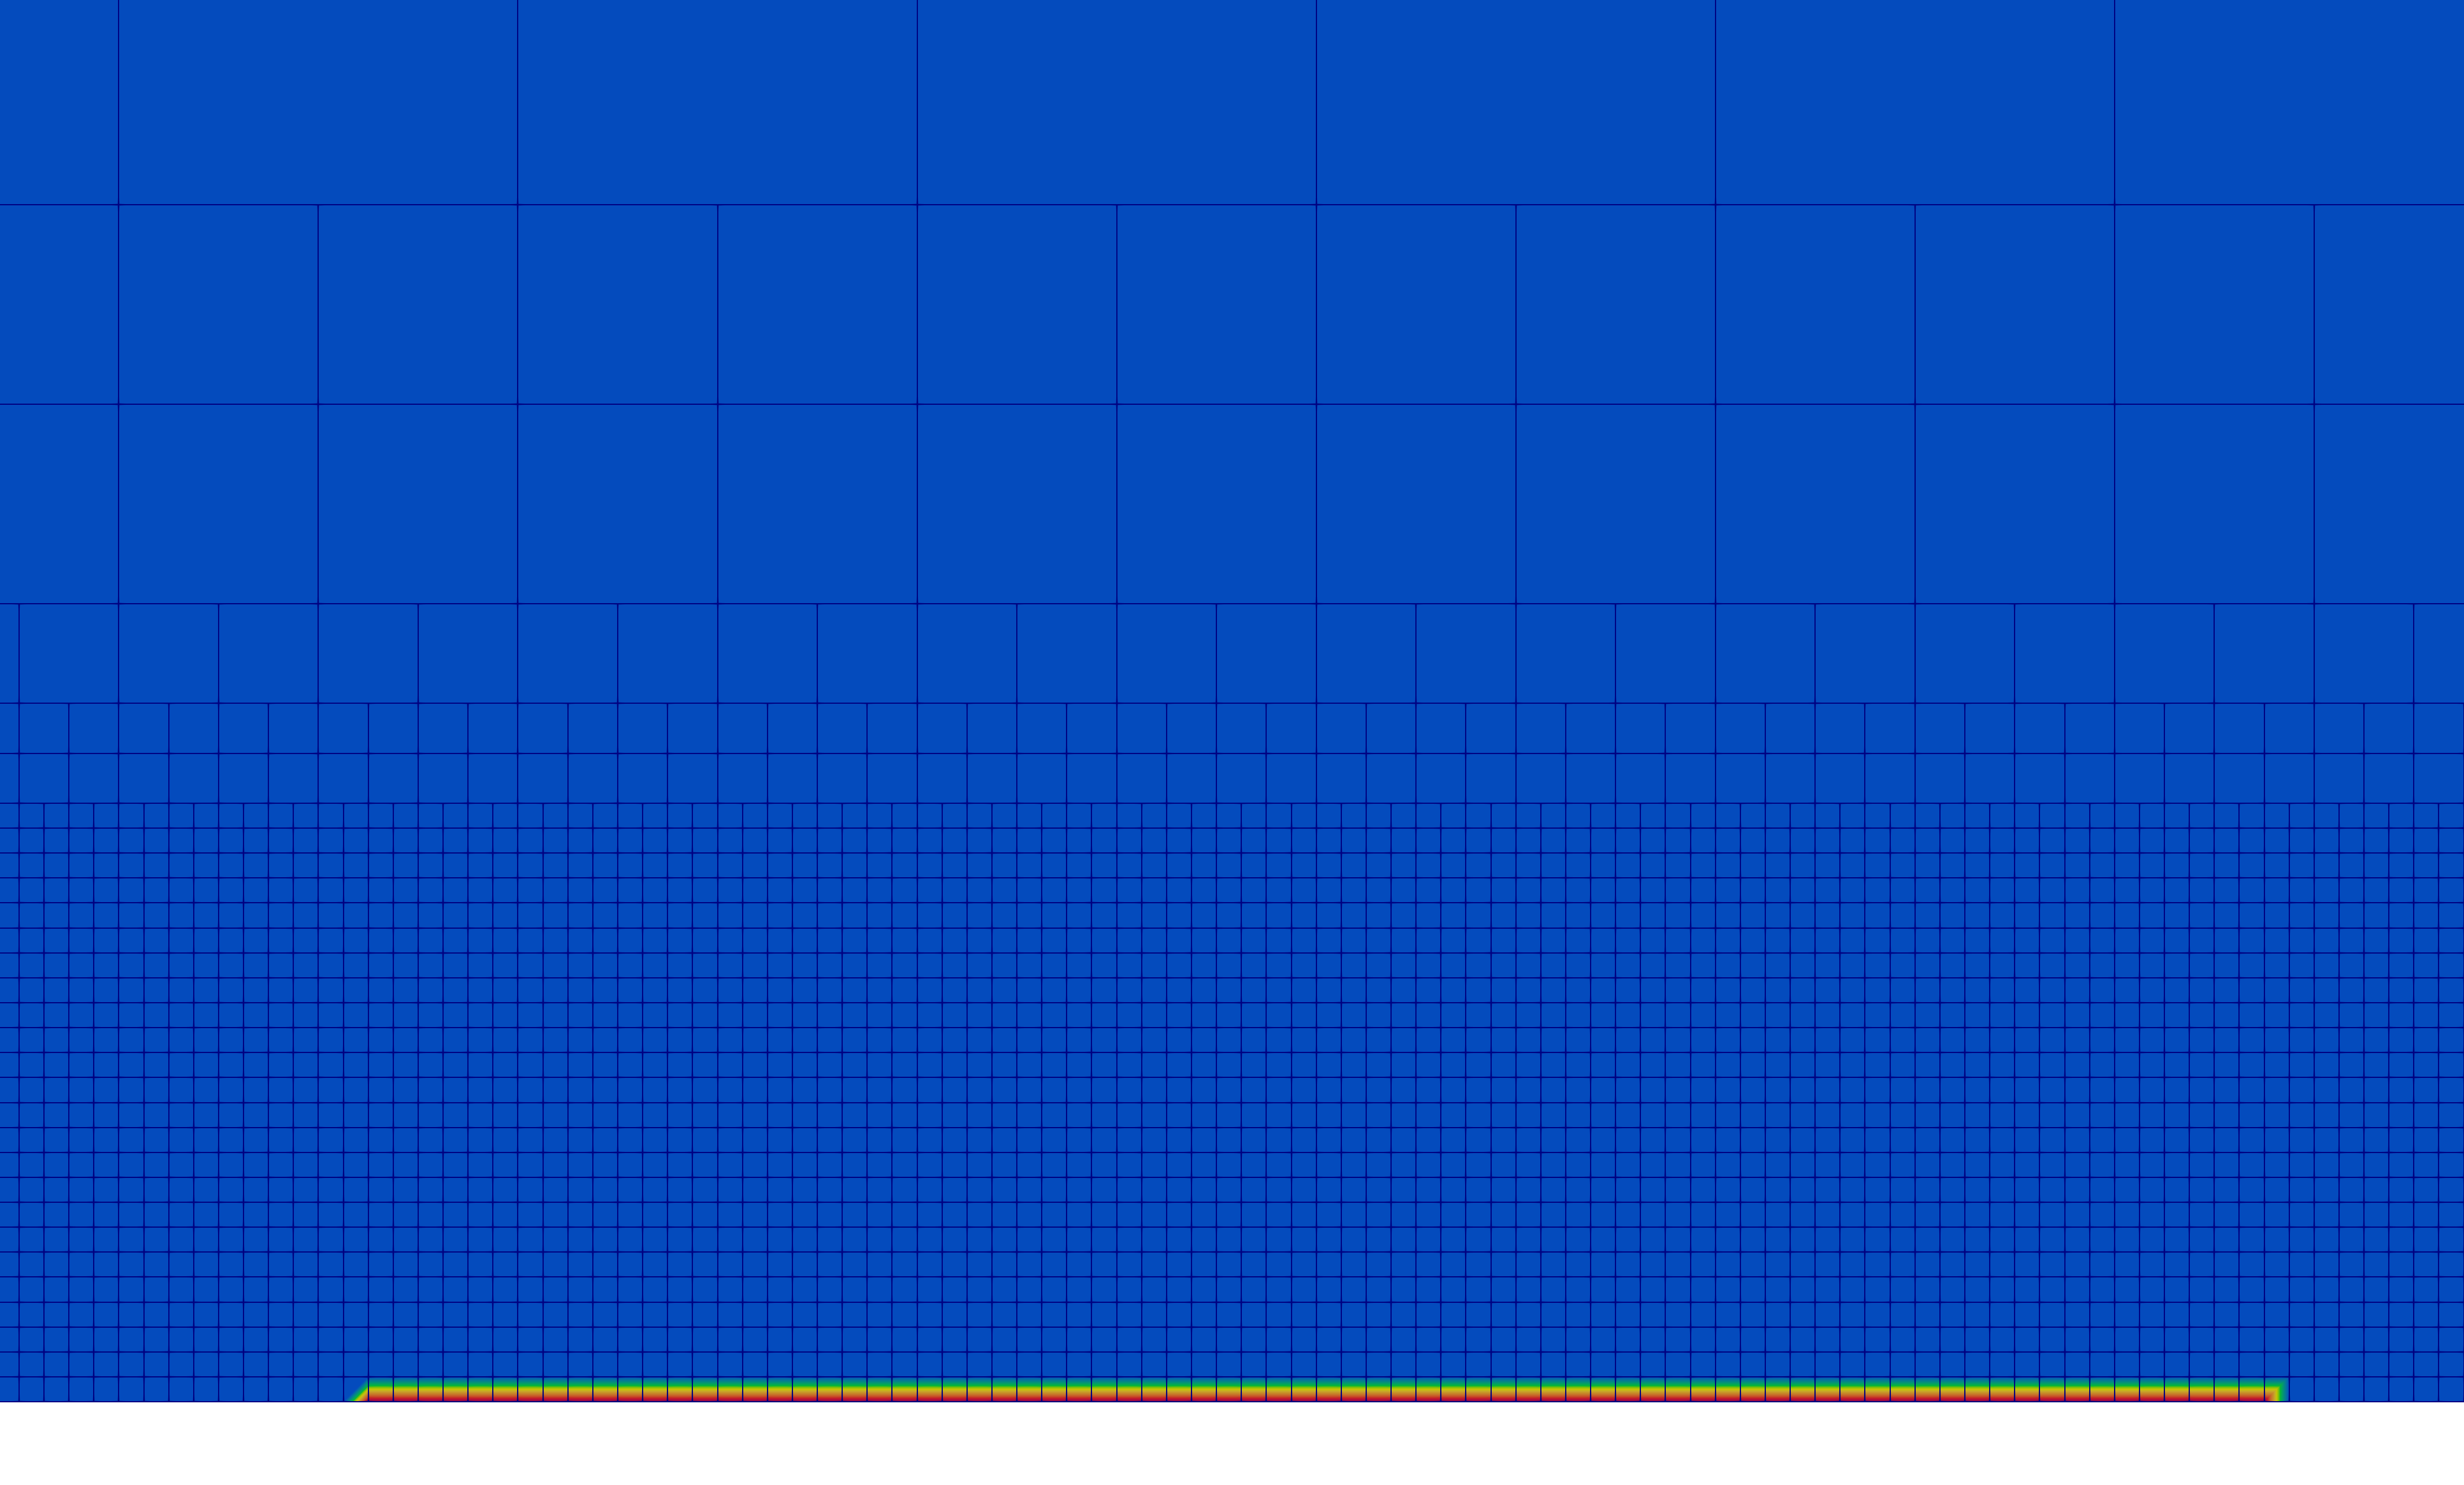
\includegraphics[width=\linewidth]{Chapter3/figures/sneddon_c0}
    \caption{}
    \label{fig:sneddon_c0}
  \end{subfigure}
  \begin{subfigure}[t]{0.46\linewidth}
    \centering
    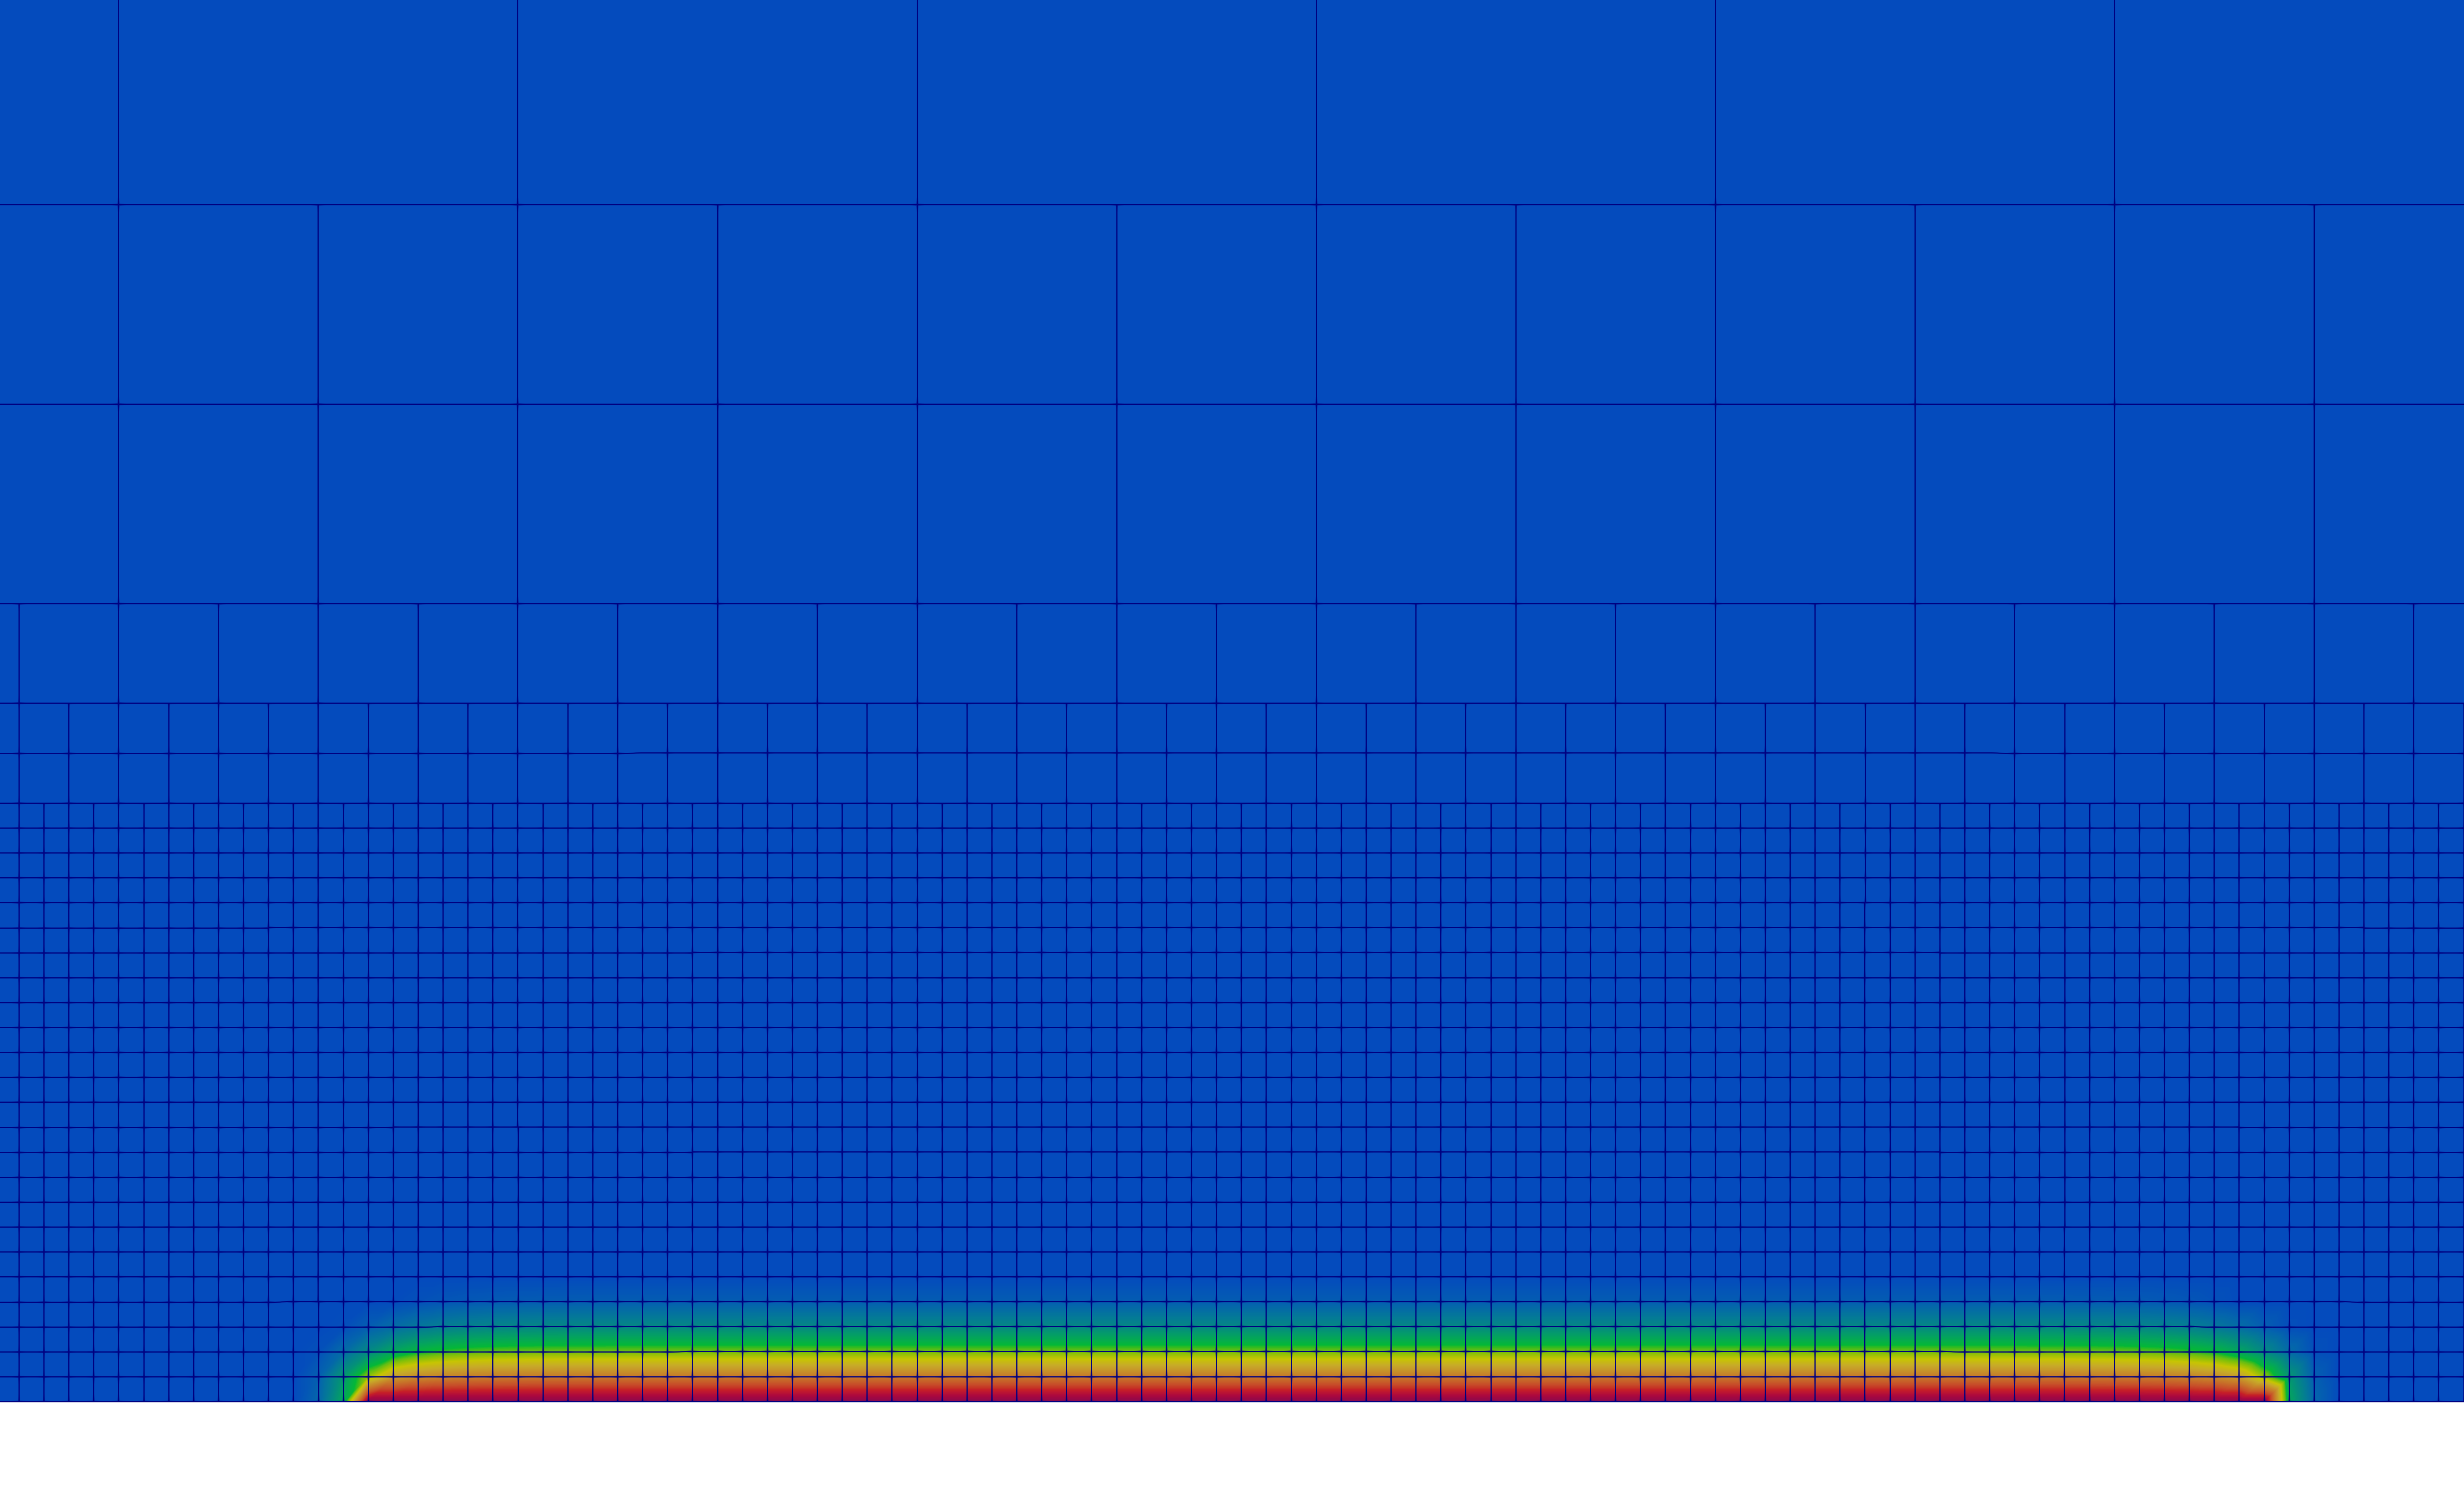
\includegraphics[width=\linewidth]{Chapter3/figures/sneddon_c1}
    \caption{}
    \label{fig:sneddon_c1}
  \end{subfigure}
  \begin{subfigure}[t]{0.475\linewidth}
    \centering
    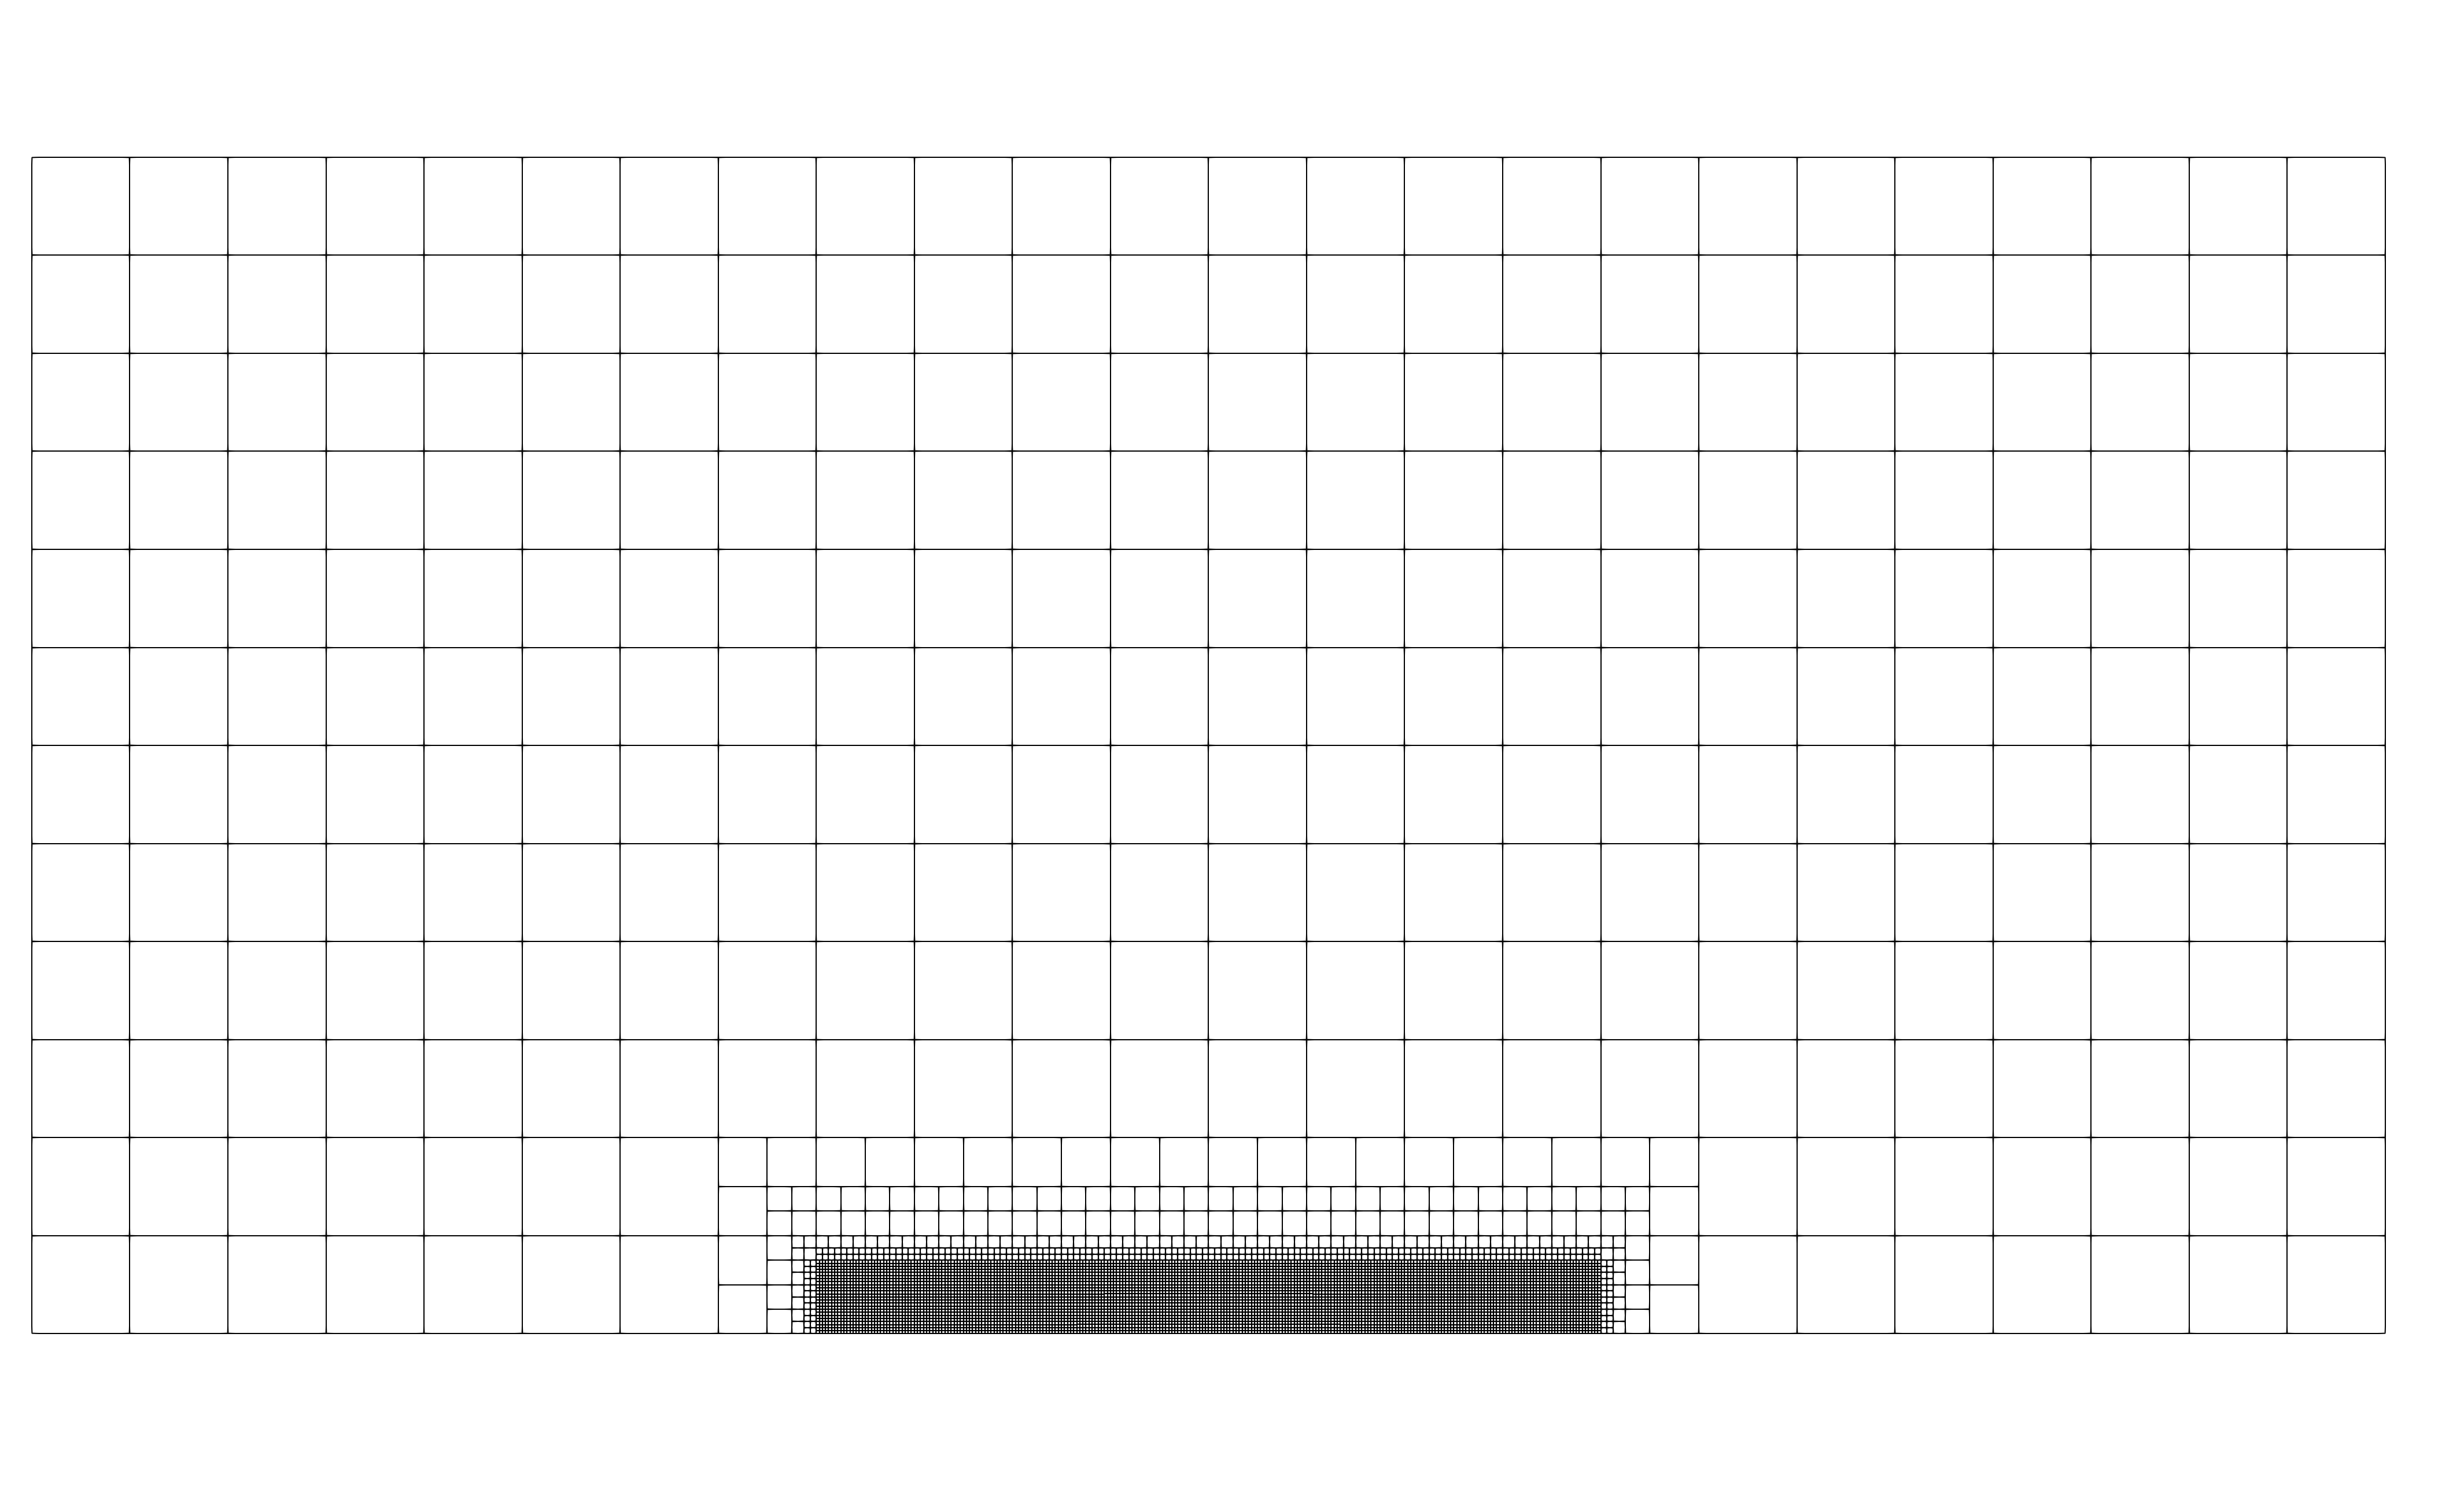
\includegraphics[width=\linewidth]{Chapter3/figures/sneddon_mesh}
    \caption{}
    \label{fig:sneddon_mesh}
  \end{subfigure}
  \begin{subfigure}[t]{0.475\linewidth}\centering
    
\includegraphics[width=\linewidth]{Chapter3/figures/sneddon_c}
    \caption{}
    \label{fig:sneddon_c}
  \end{subfigure}
  \caption[Sneddon benchmark problem.]{\label{fig:sneddon}Pressurized crack propagation problem: (a) Initial values are imposed on crack surface nodes (zoomed view). (b) Regularized phase-field variable after one time step (zoomed view). (c) Mesh with five levels of local refinement. (d) Pre-existing crack. The red and blue color correspond to value of 1.0 and 0, respectively.}
\end{figure}

\begin{figure}[!ht]
  \centering
  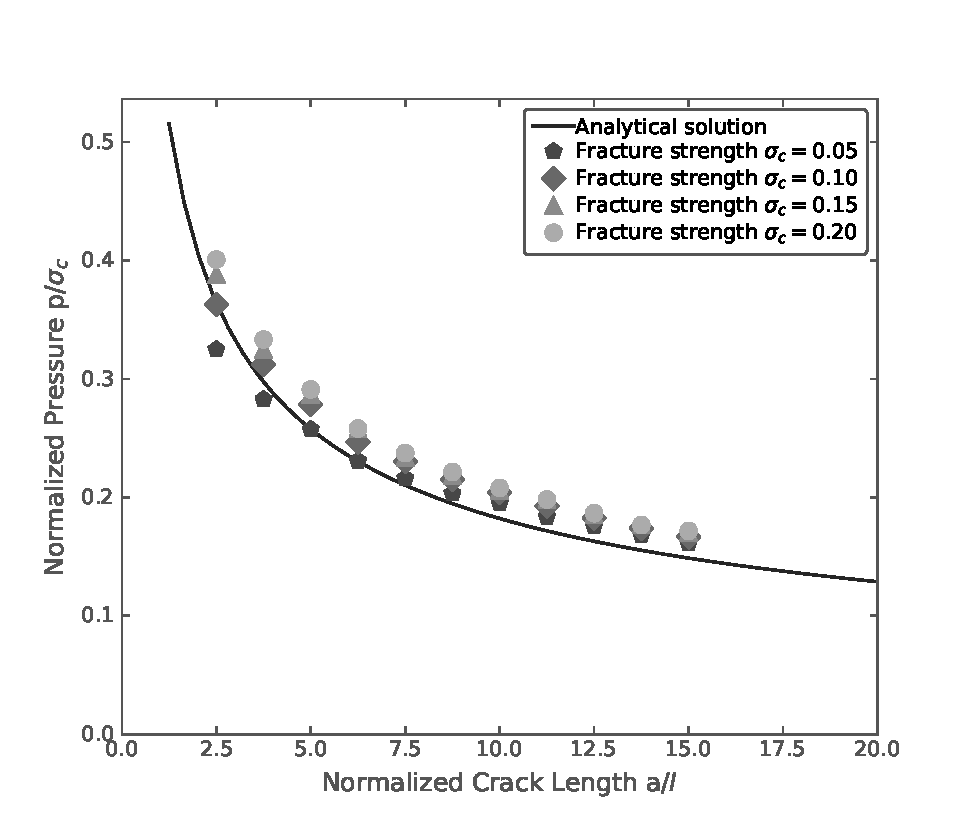
\includegraphics[width=0.6\textwidth]{Chapter3/figures/critical_pressure}
  \caption{Comparison between the numerical results and the LEFM solution for the critical pressure values.}
  \label{fig:critical_presssure}
\end{figure}
